\newpage
\section*{Biomarker Discovery}

\begin{figure}[H]
  \caption{Biomarkers at Conserved 200kb and 400kb Domain Boundaries}\label{fig:boundaryBiomarkers}
  \begin{minipage}{0.5\textwidth}%
    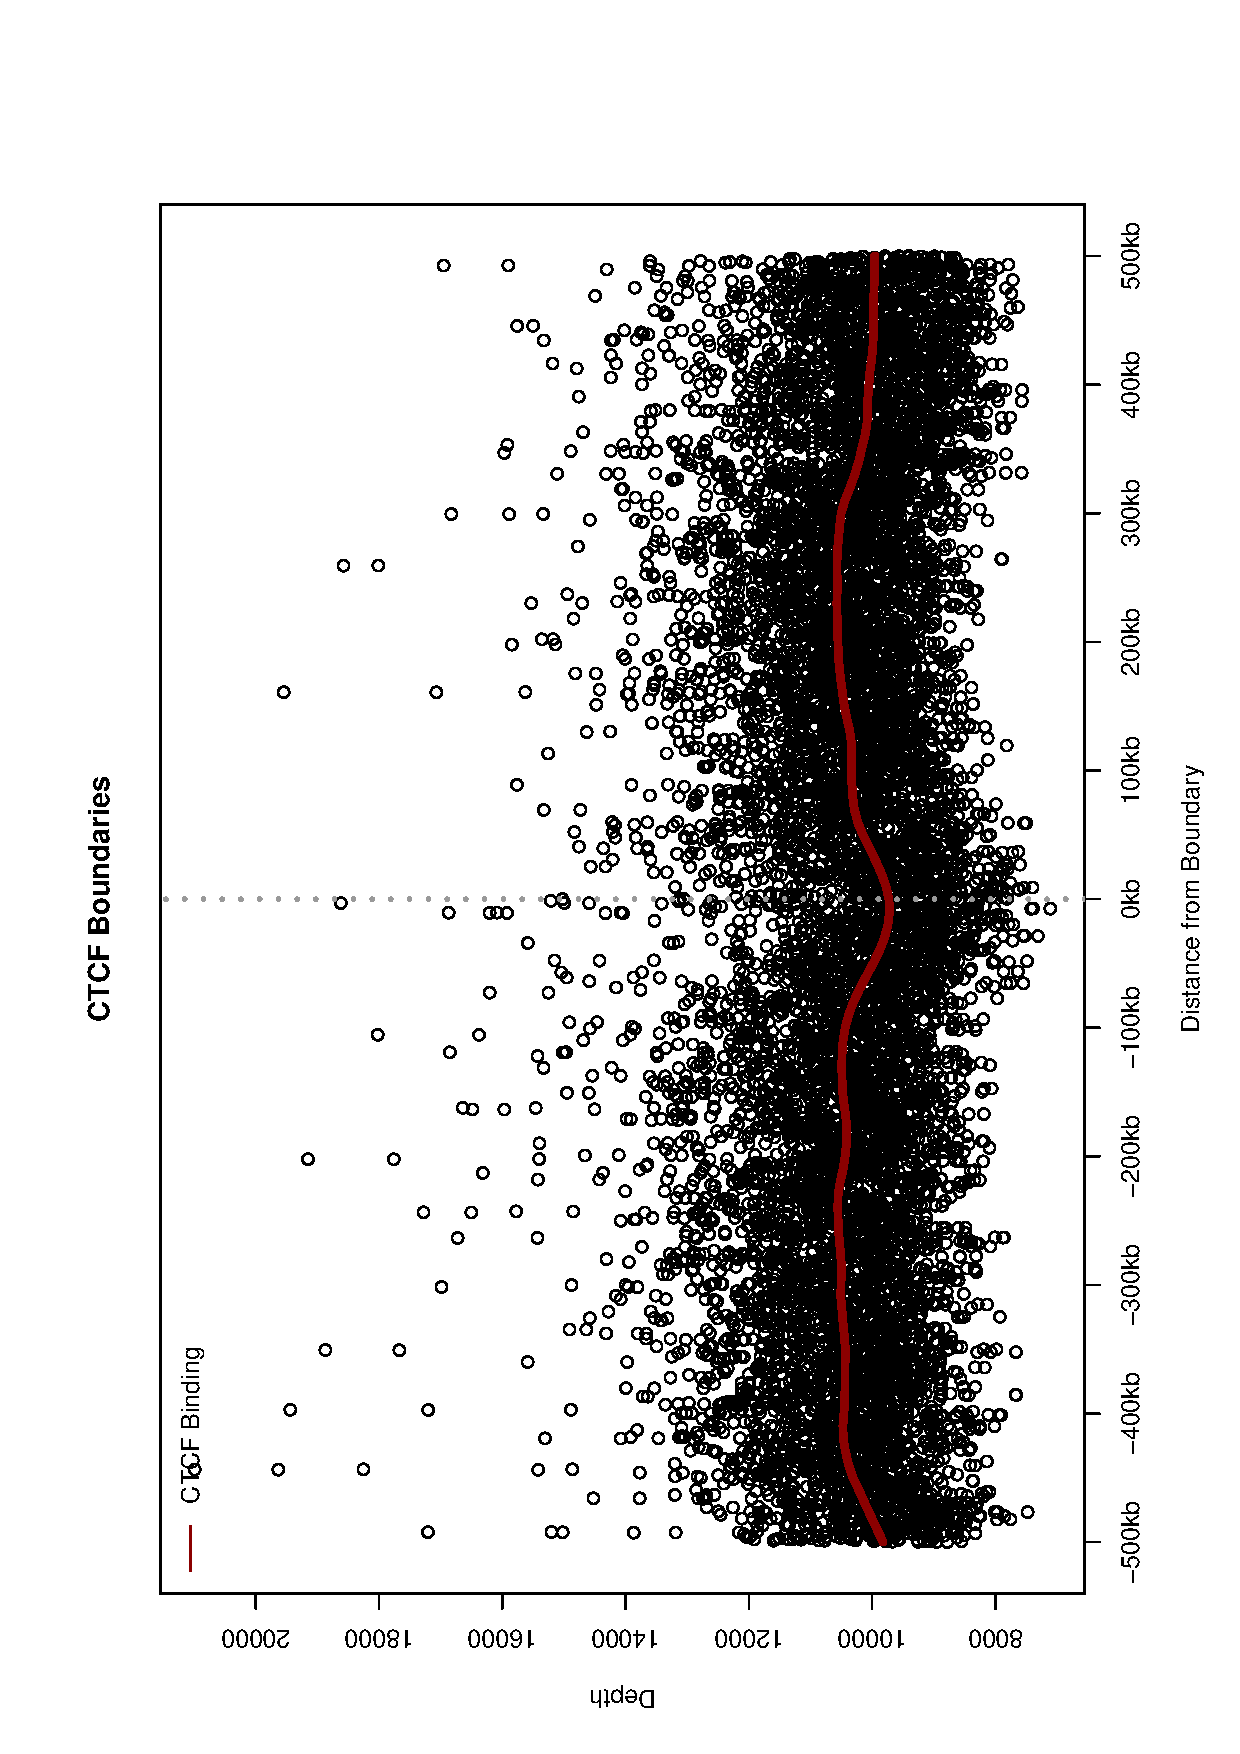
\includegraphics[width=\textwidth]{./figures/supplementary/biomarkers/ctcf200kbboundaries.pdf}
  \end{minipage}%
  \hfill
  \begin{minipage}{0.5\textwidth}
    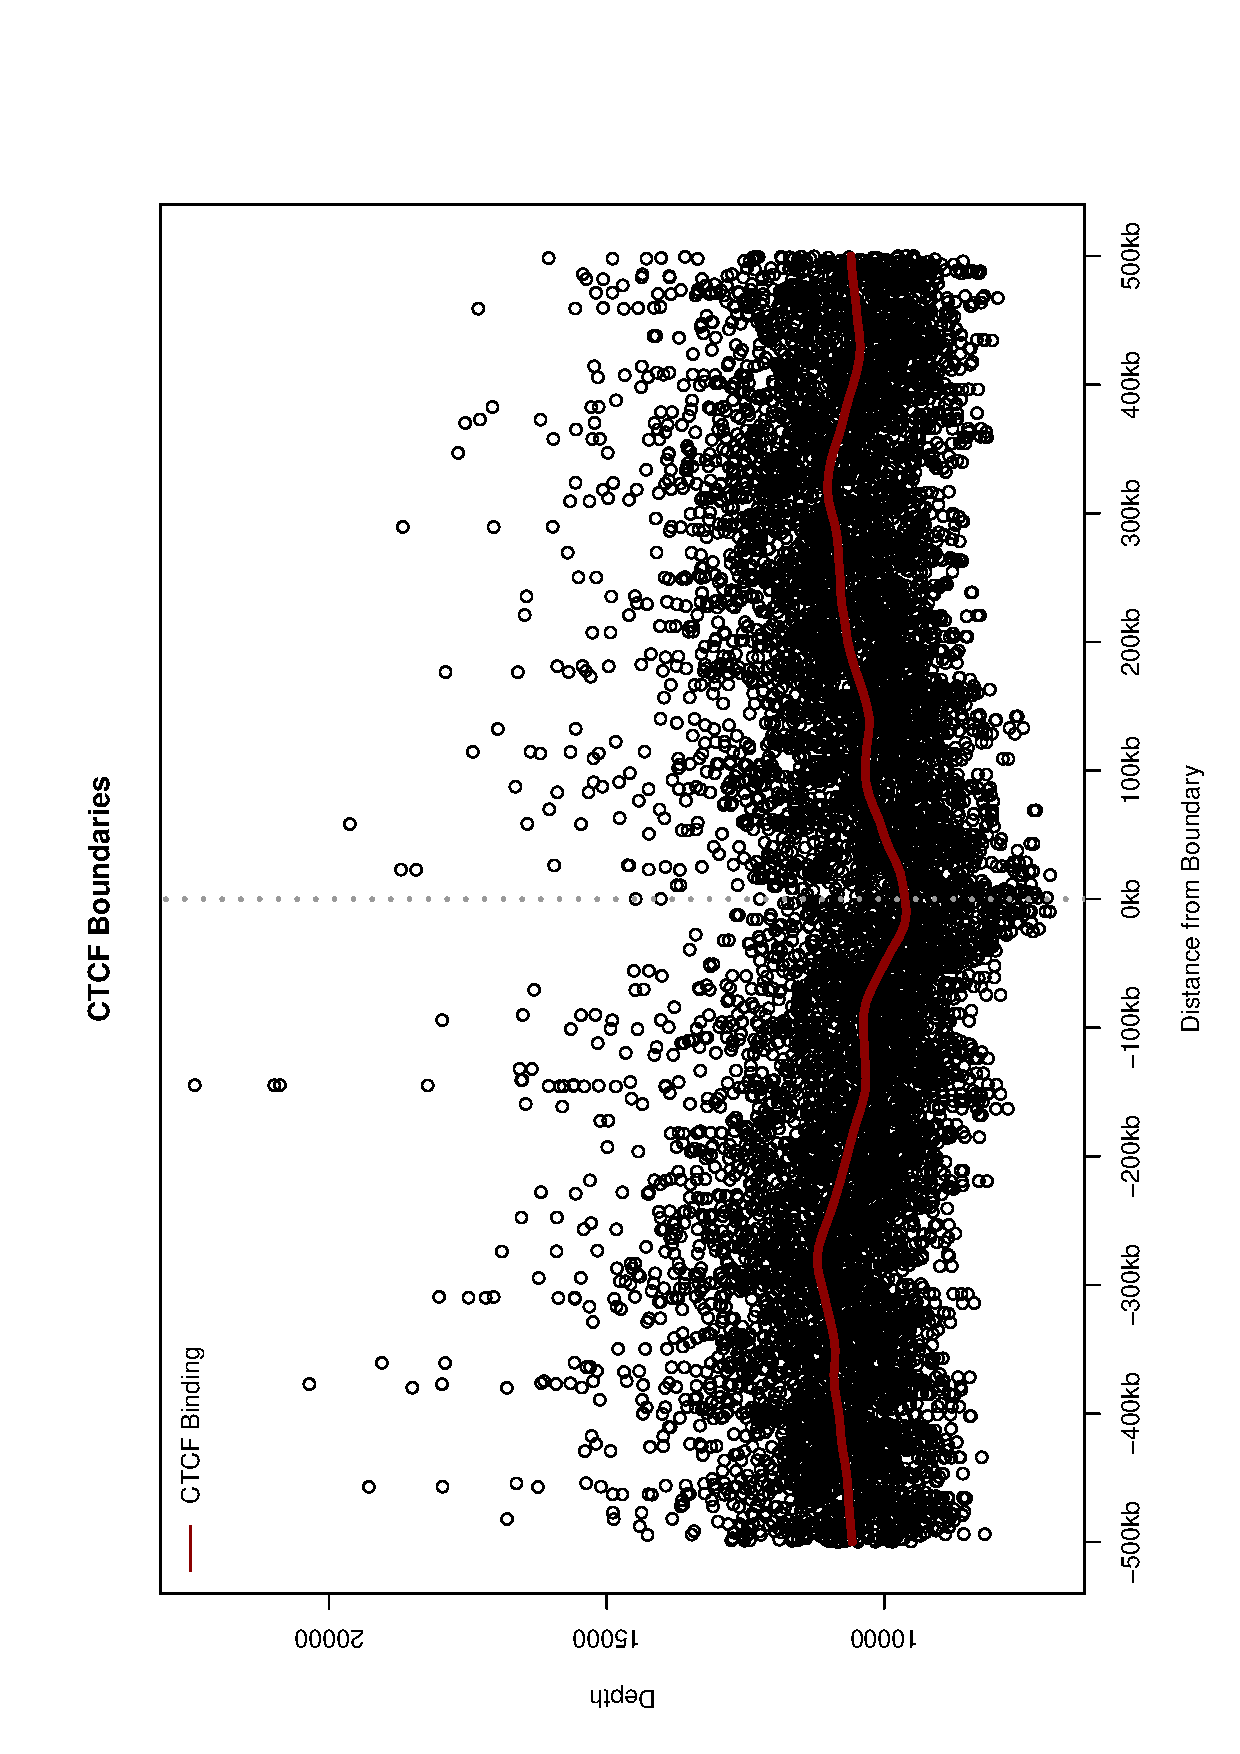
\includegraphics[width=\textwidth]{./figures/supplementary/biomarkers/ctcf400kbboundaries.pdf}
  \end{minipage}
\end{figure}

\begin{figure}[H]
  \begin{minipage}{0.5\textwidth}%
    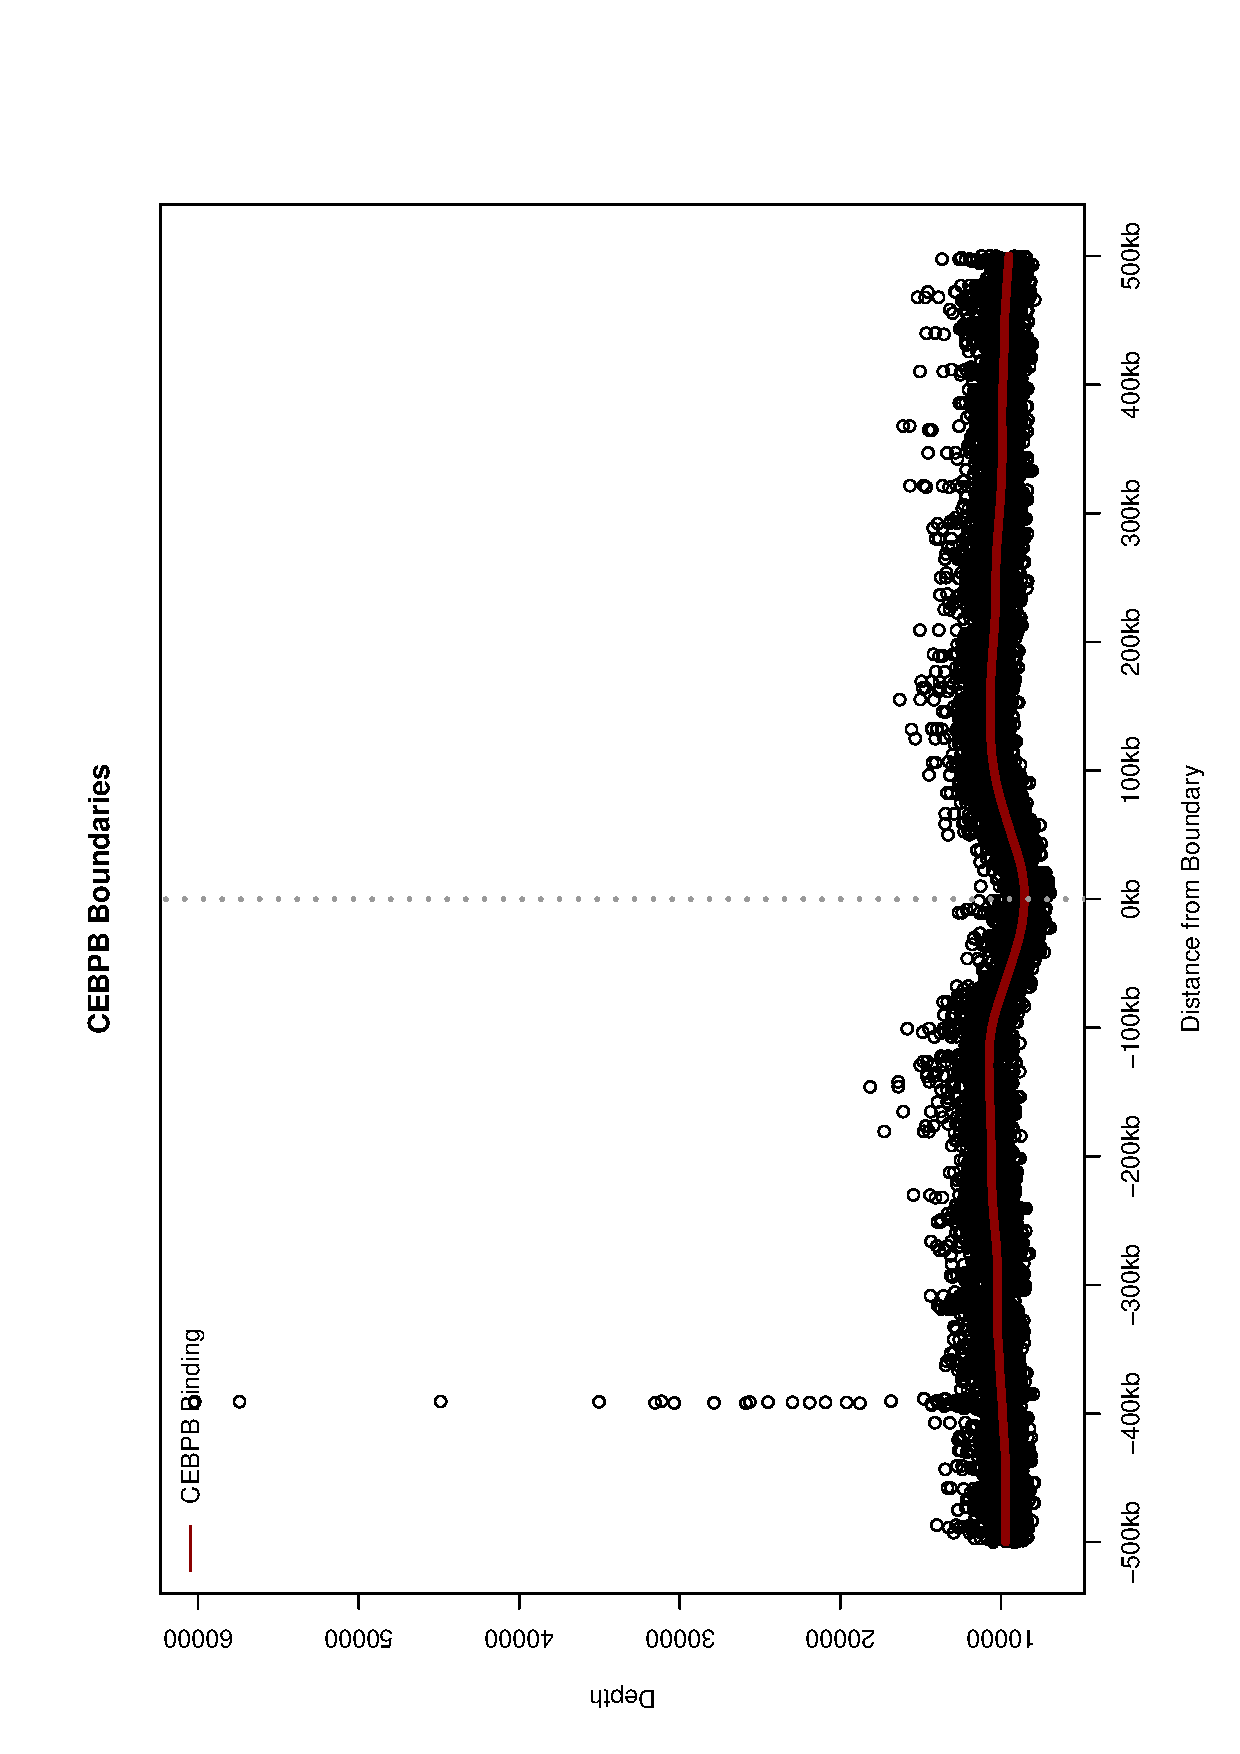
\includegraphics[width=\textwidth]{./figures/supplementary/biomarkers/cebpb200kbboundaries.pdf}
  \end{minipage}%
  \hfill
  \begin{minipage}{0.5\textwidth}
    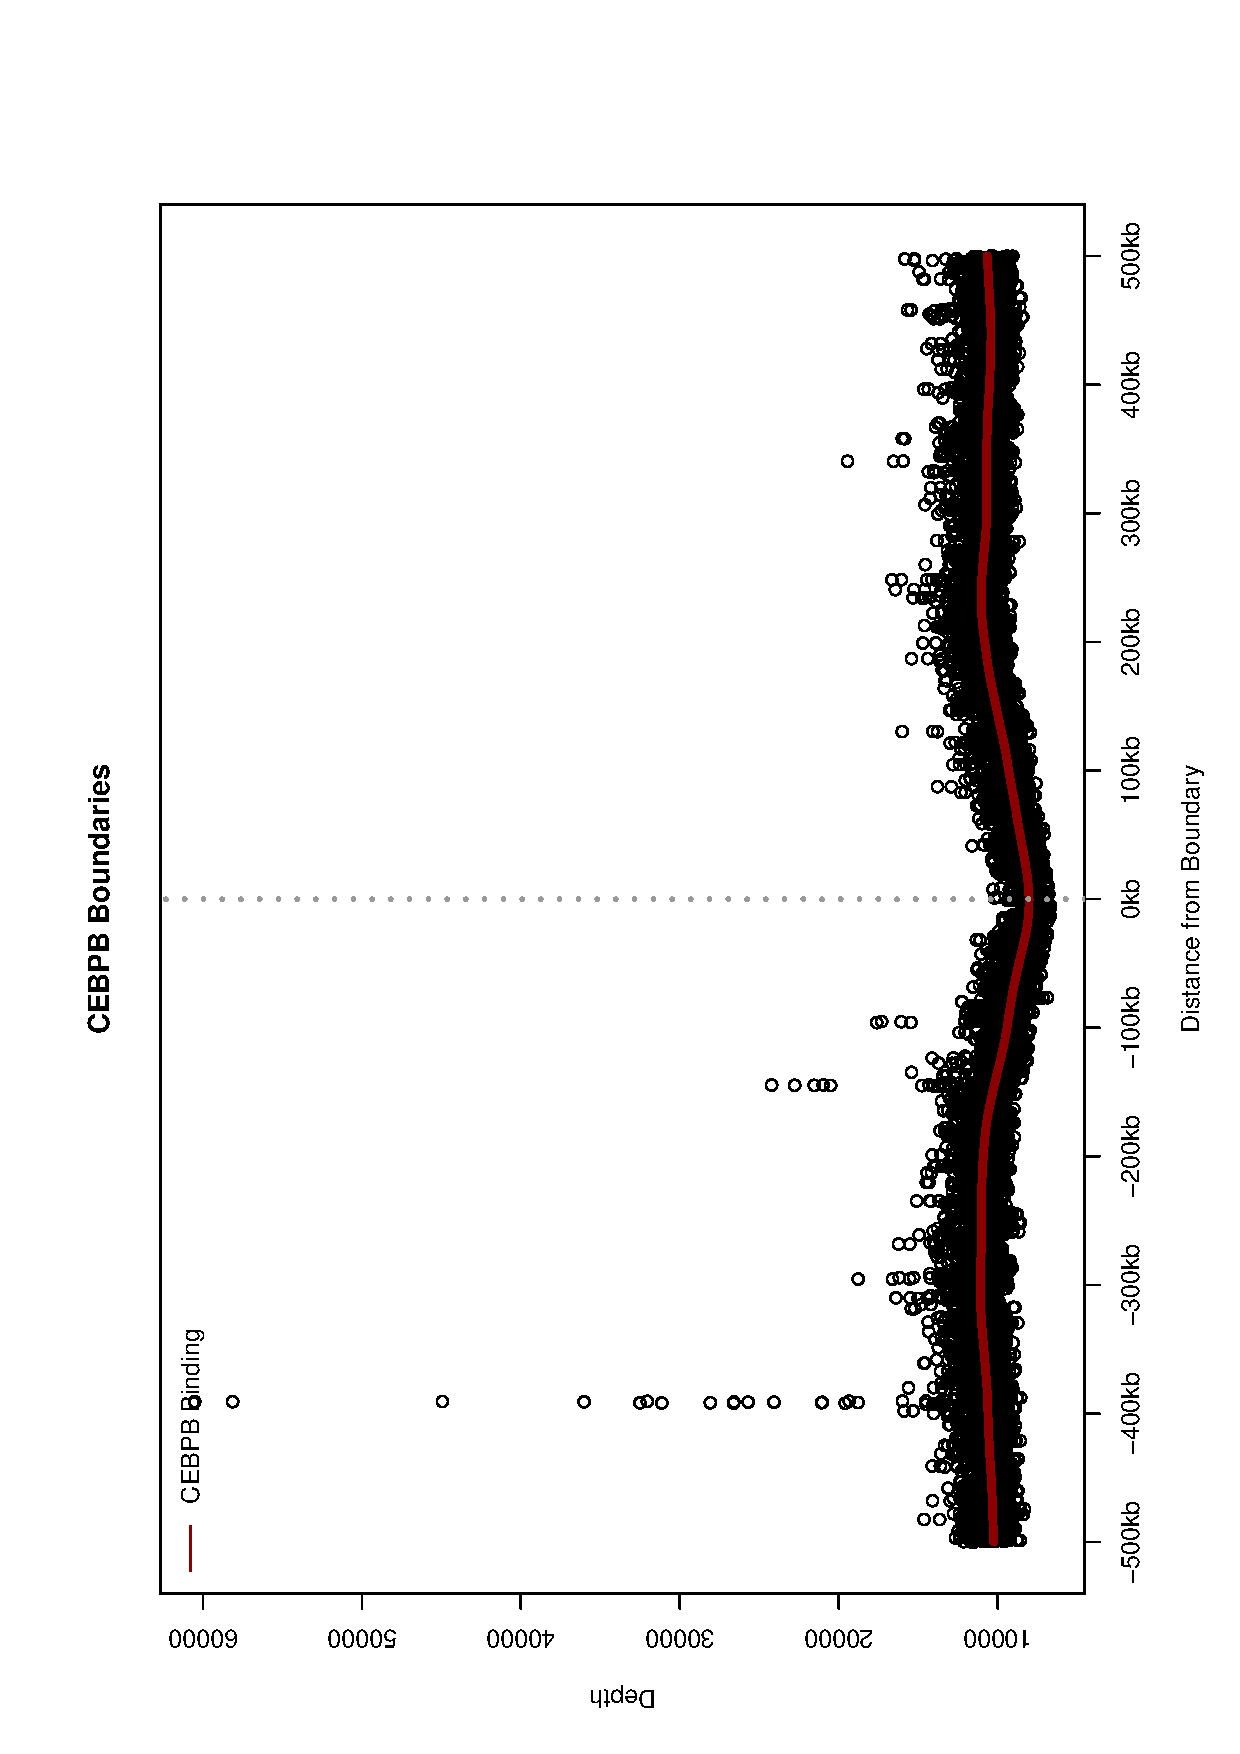
\includegraphics[width=\textwidth]{./figures/supplementary/biomarkers/cebpb400kbboundaries.pdf}
  \end{minipage}
\end{figure}

\begin{figure}[H]
  \begin{minipage}{0.5\textwidth}%
    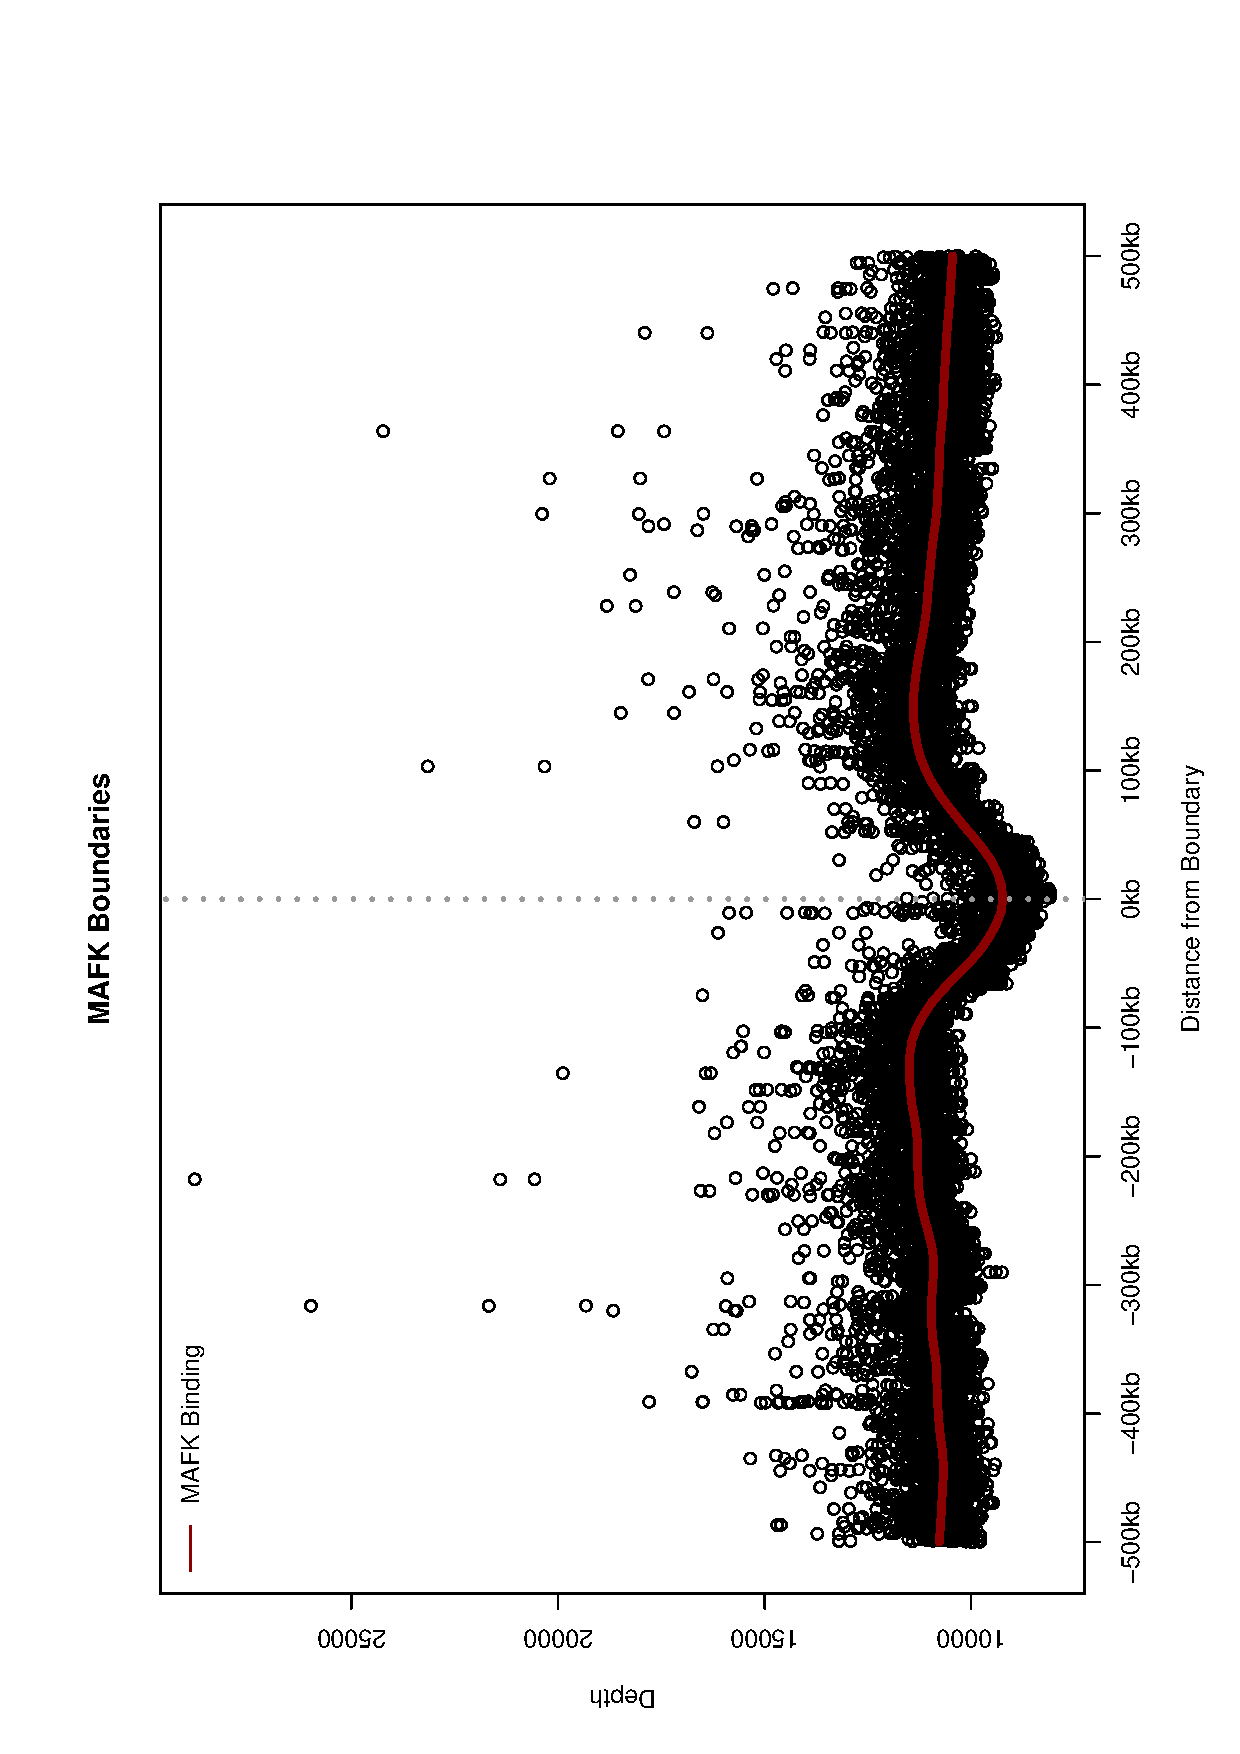
\includegraphics[width=\textwidth]{./figures/supplementary/biomarkers/mafk200kbboundaries.pdf}
  \end{minipage}%
  \hfill
  \begin{minipage}{0.5\textwidth}
    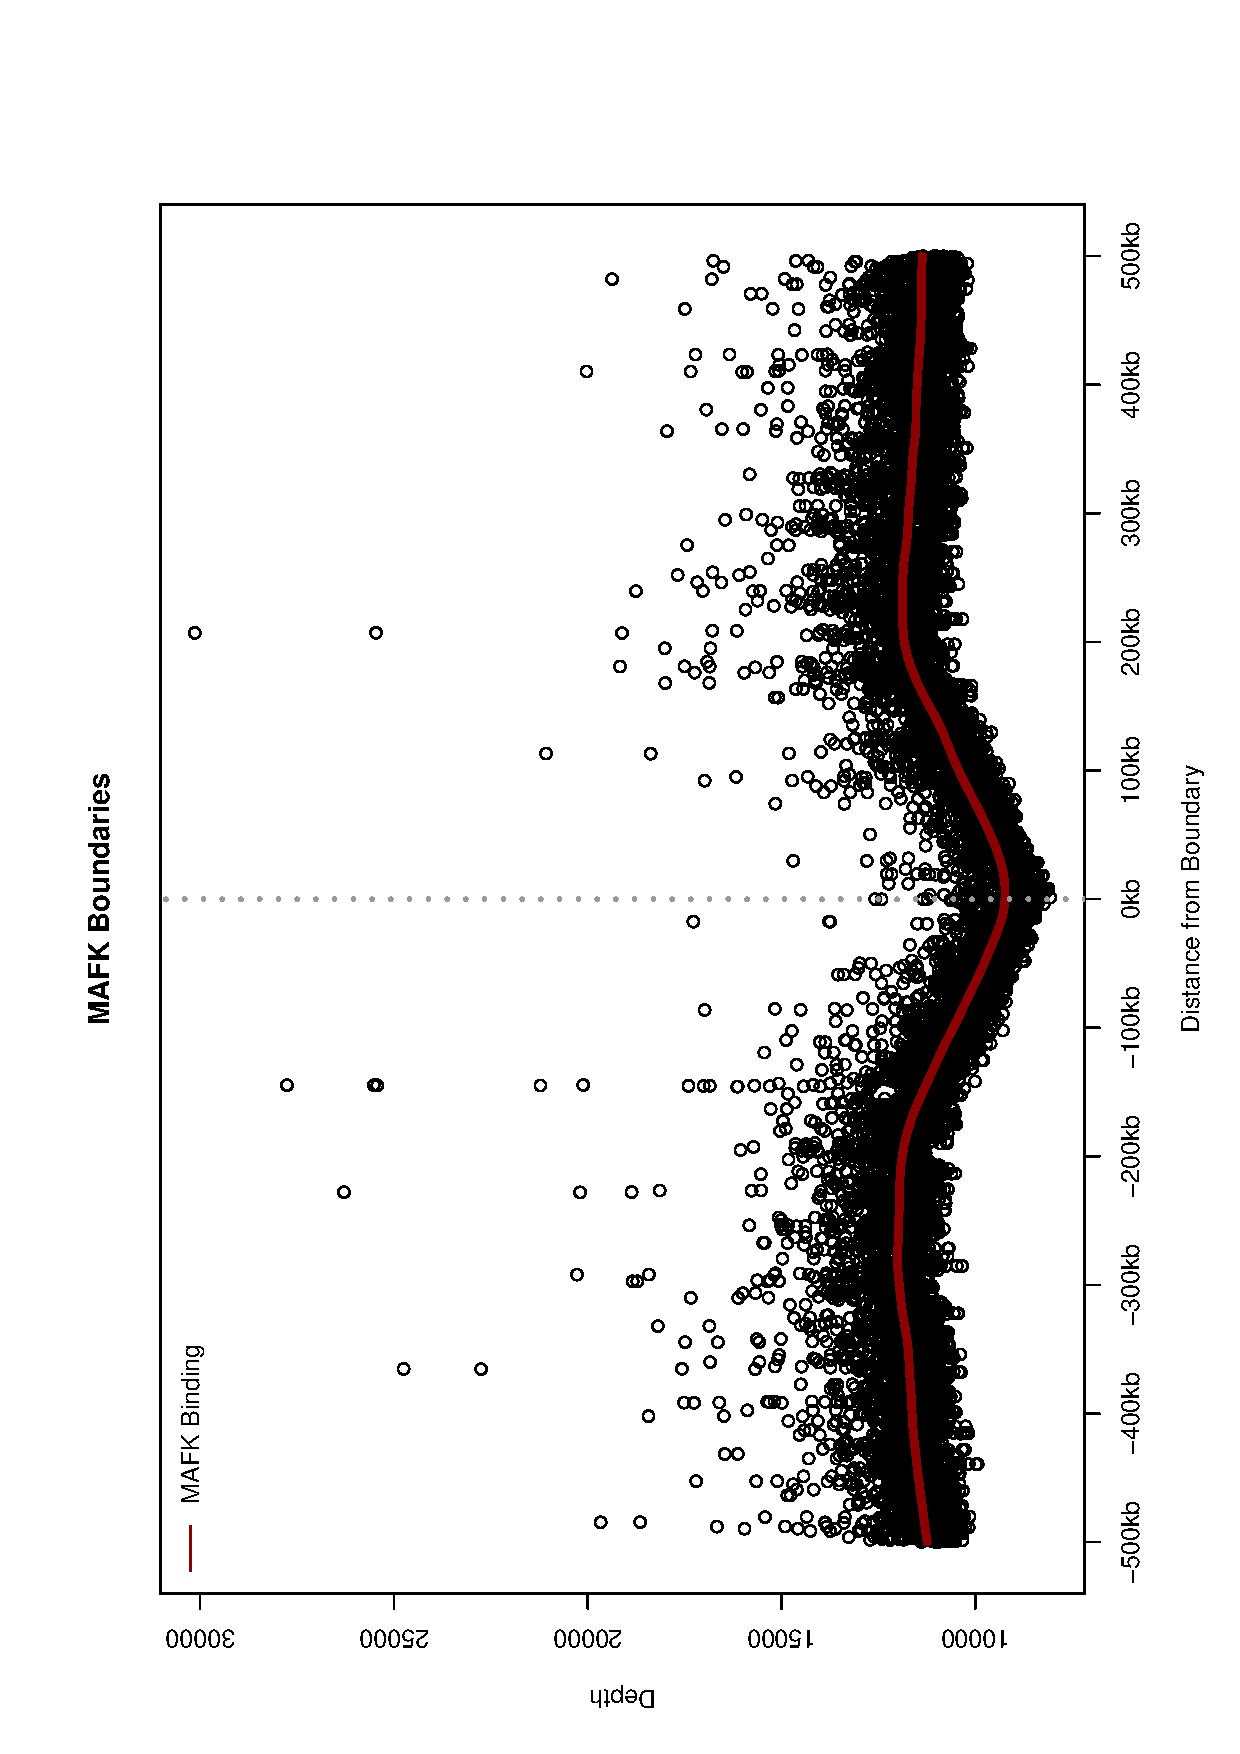
\includegraphics[width=\textwidth]{./figures/supplementary/biomarkers/mafk400kbboundaries.pdf}
  \end{minipage}
\end{figure}

\begin{figure}[H]
  \begin{minipage}{0.5\textwidth}%
    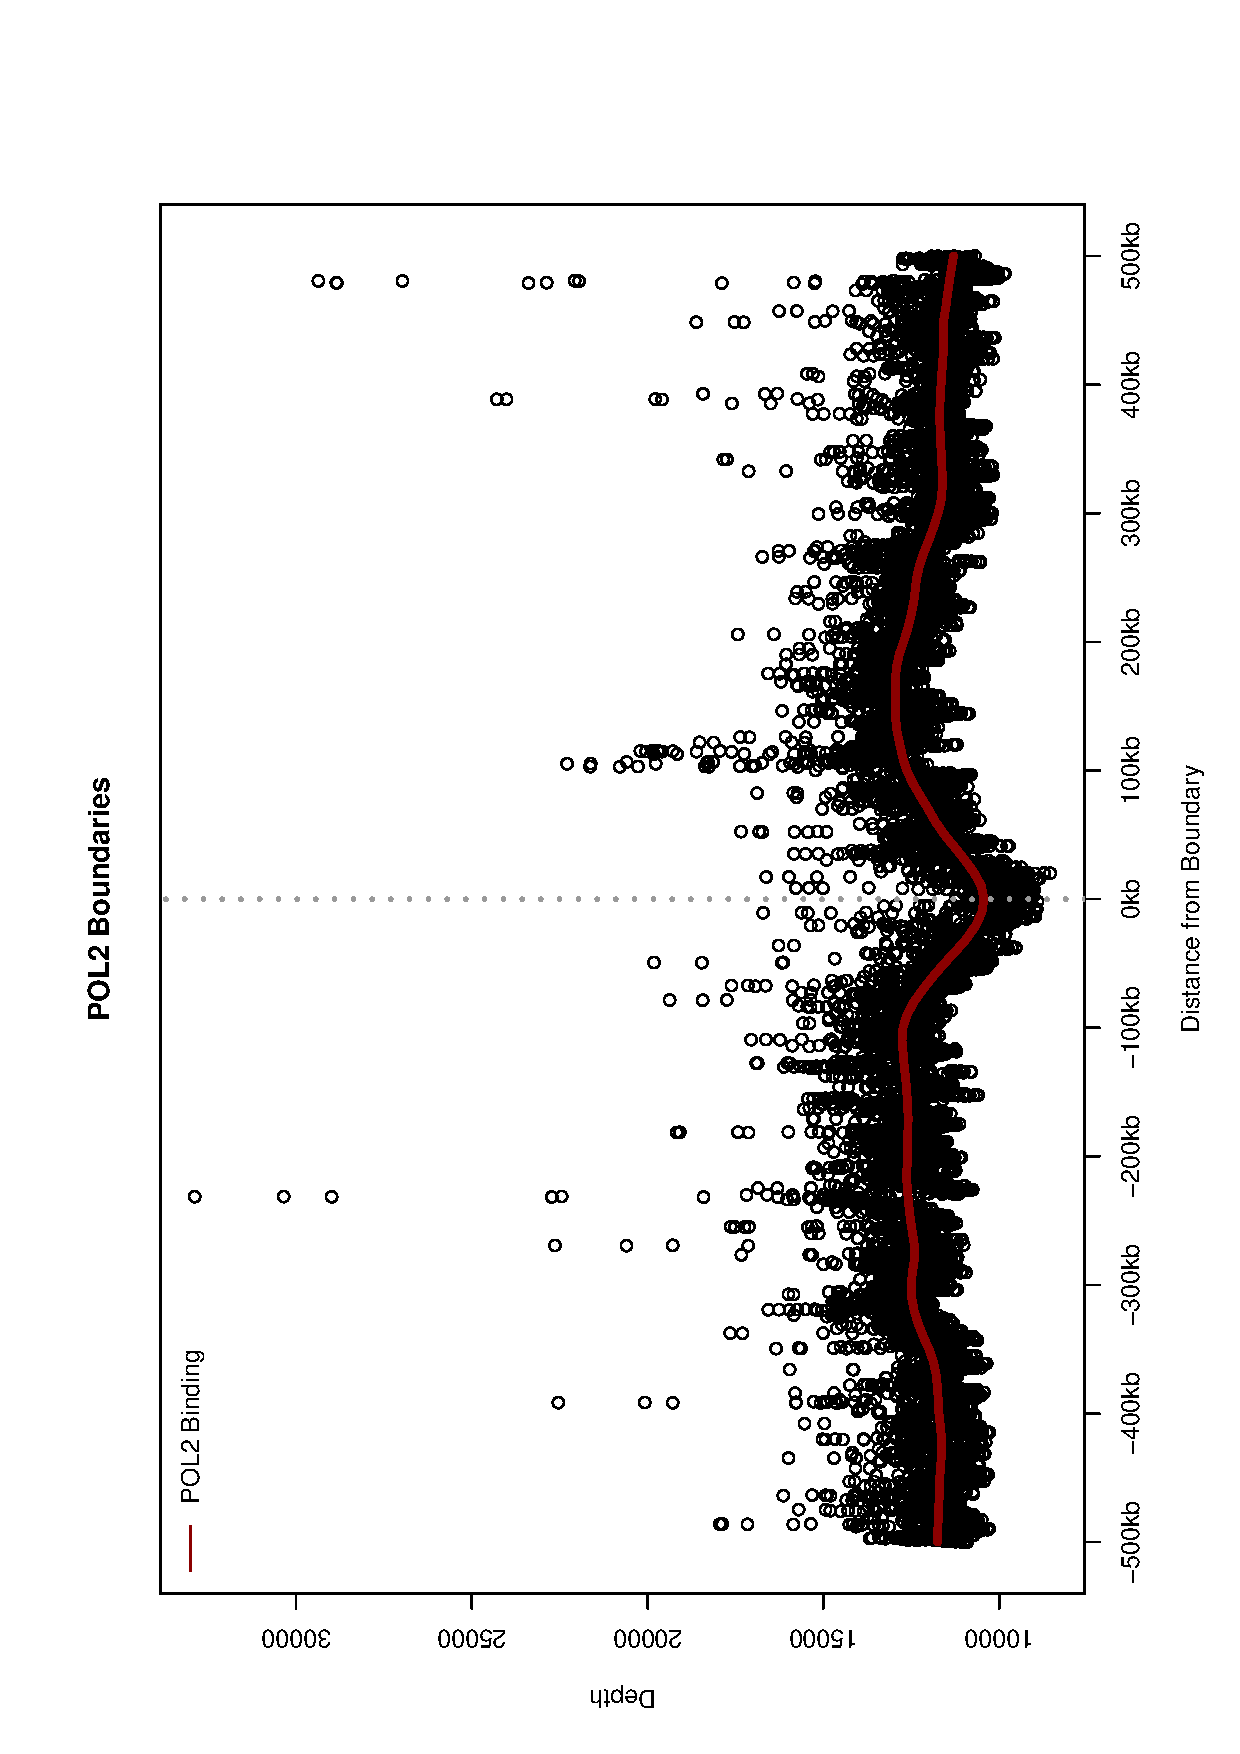
\includegraphics[width=\textwidth]{./figures/supplementary/biomarkers/pol2200kbboundaries.pdf}
  \end{minipage}%
  \hfill
  \begin{minipage}{0.5\textwidth}
    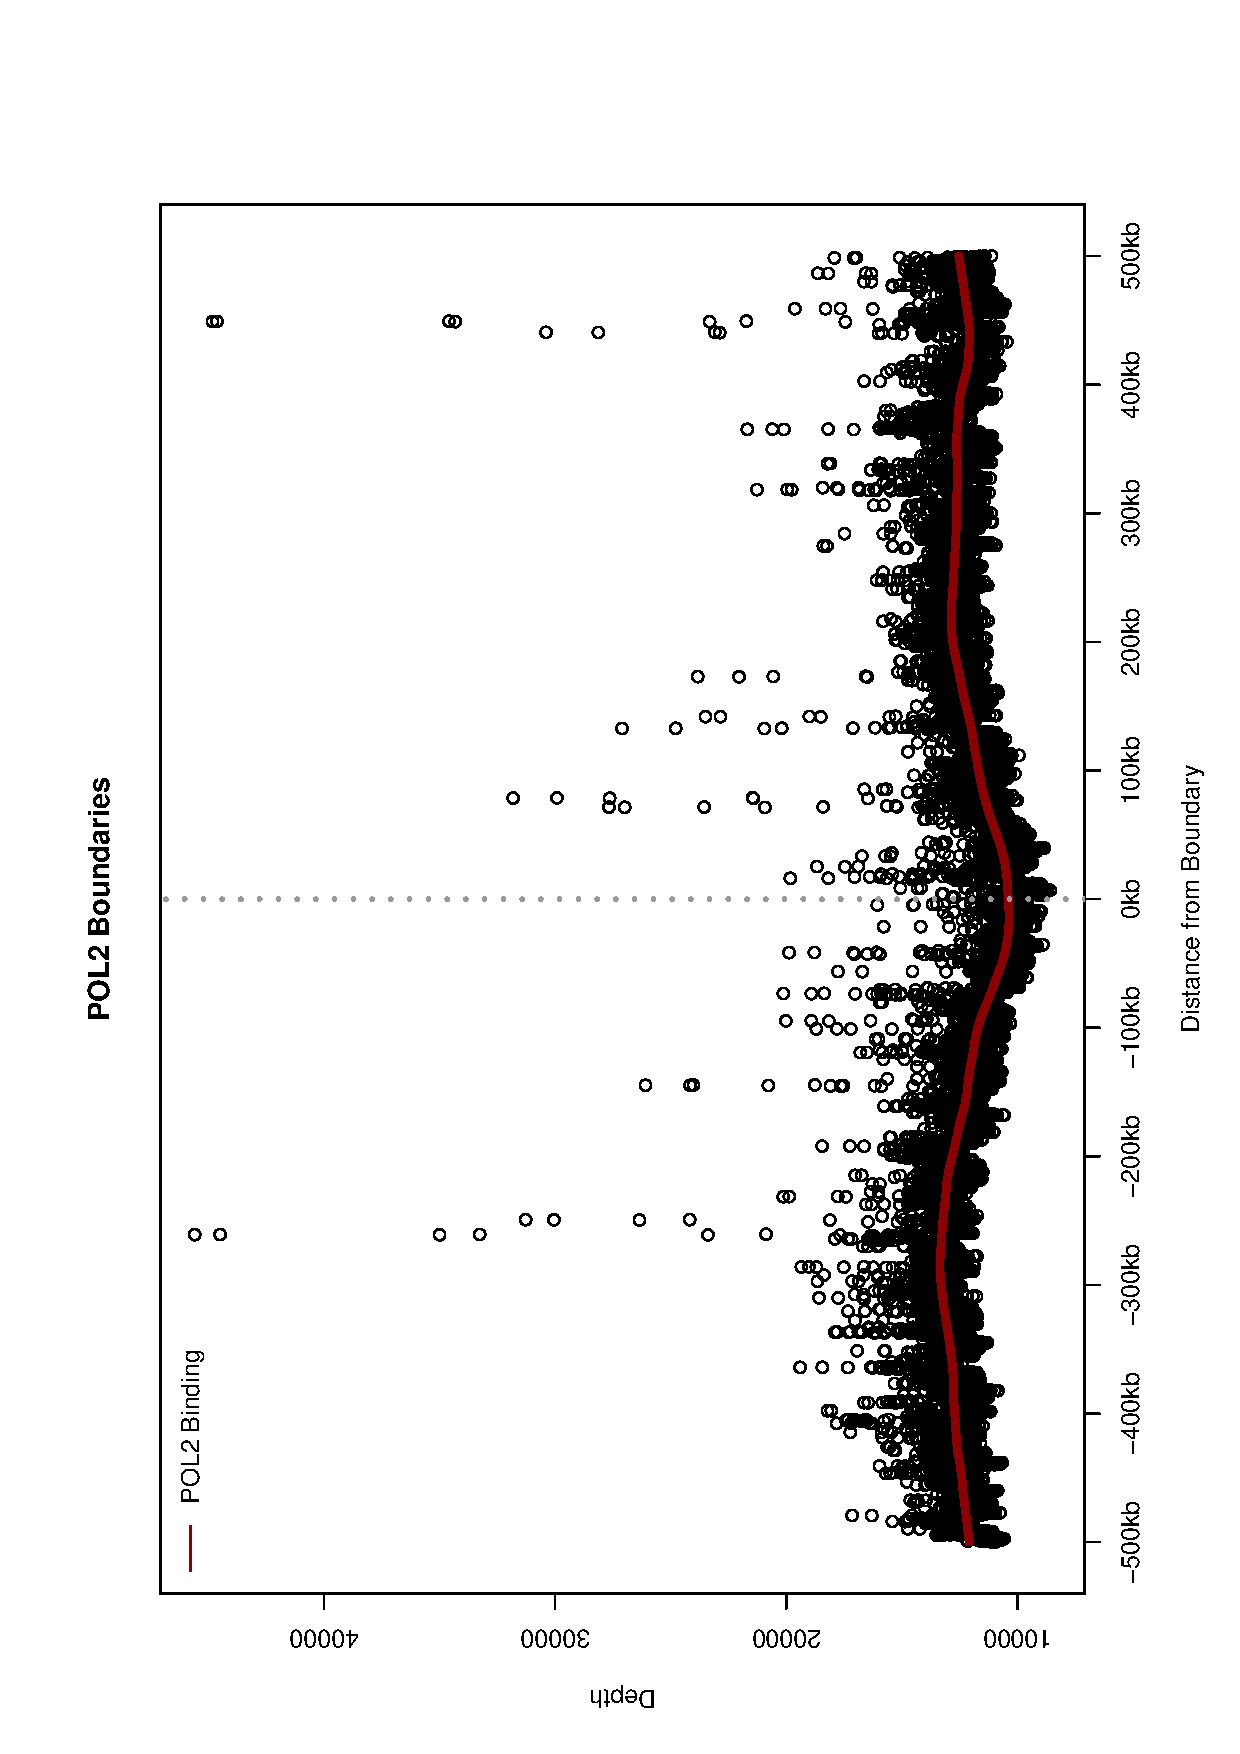
\includegraphics[width=\textwidth]{./figures/supplementary/biomarkers/pol2400kbboundaries.pdf}
  \end{minipage}
\end{figure}

\begin{figure}[H]
  \begin{minipage}{0.5\textwidth}%
    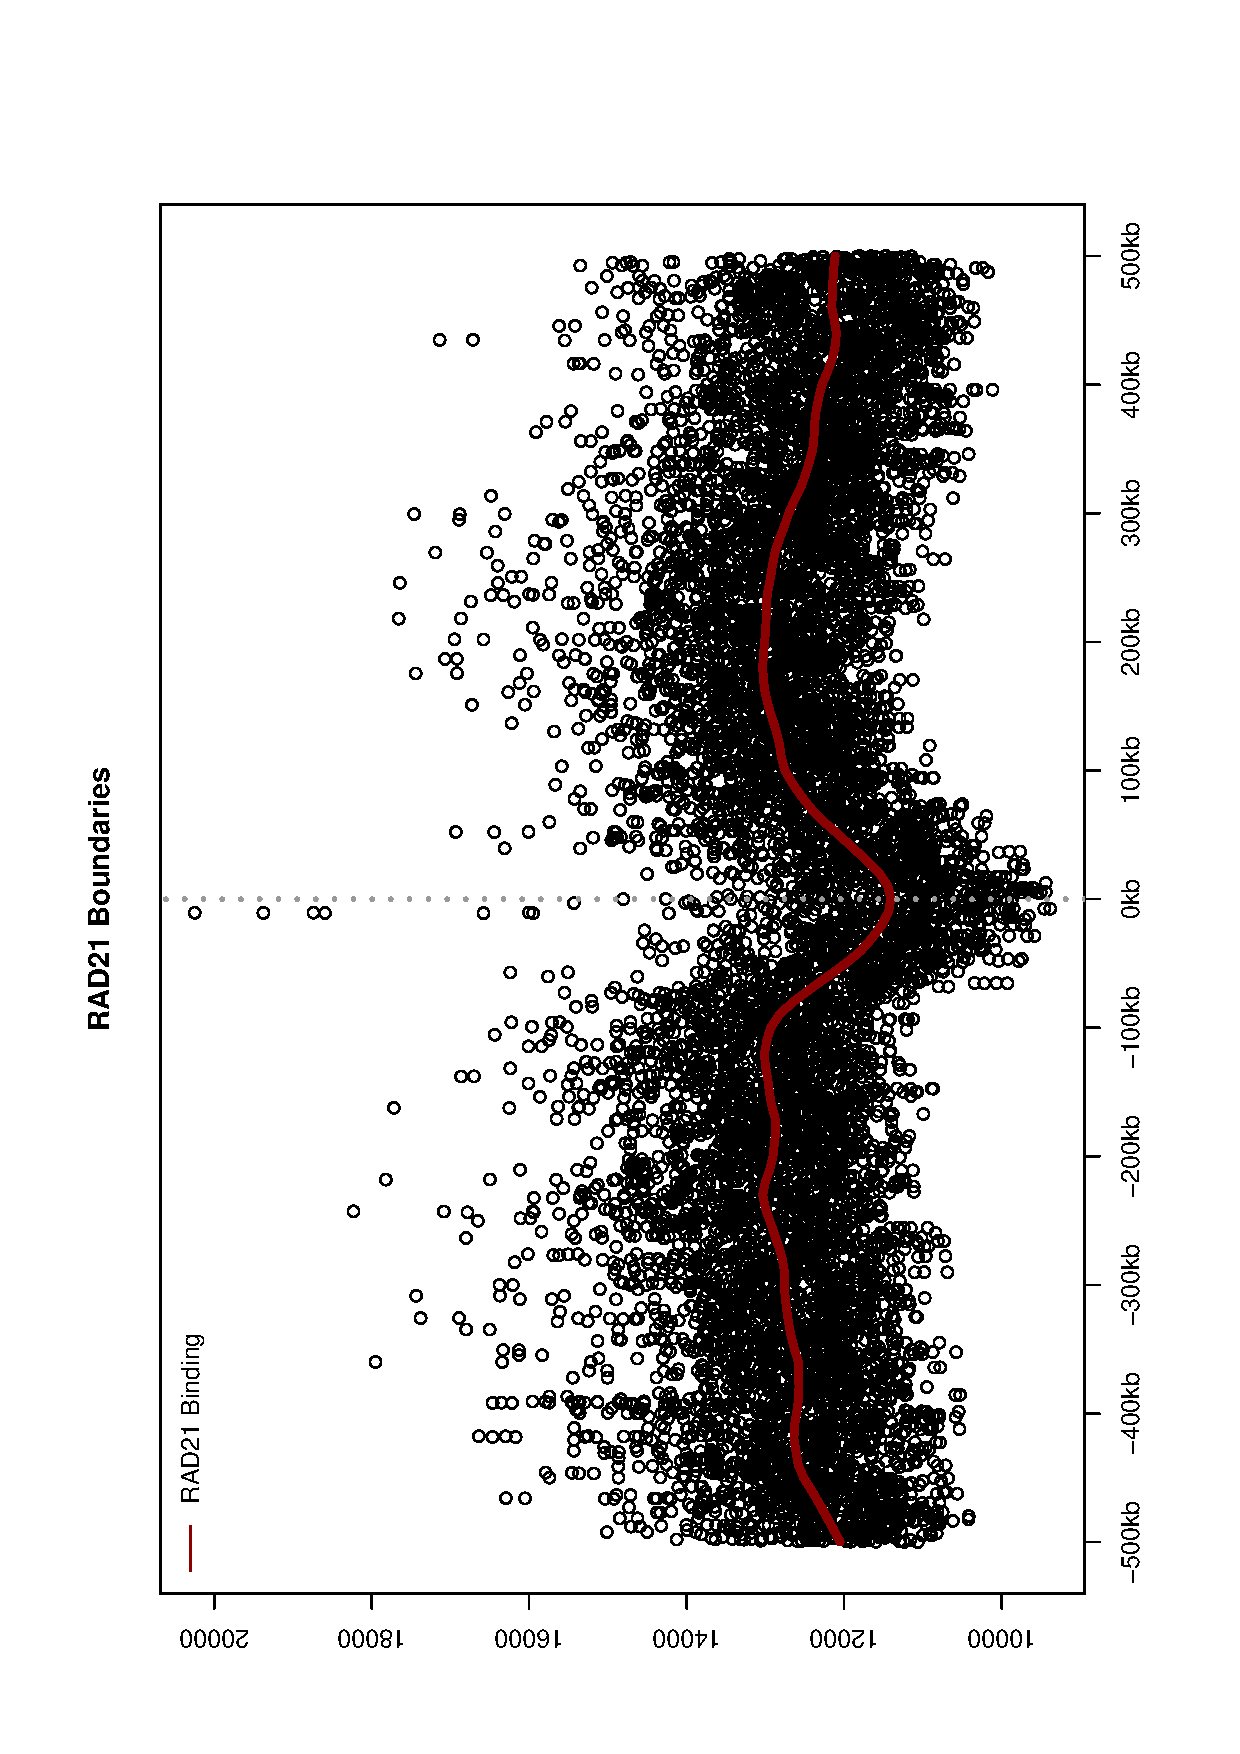
\includegraphics[width=\textwidth]{./figures/supplementary/biomarkers/rad21200kbboundaries.pdf}
  \end{minipage}%
  \hfill
  \begin{minipage}{0.5\textwidth}
    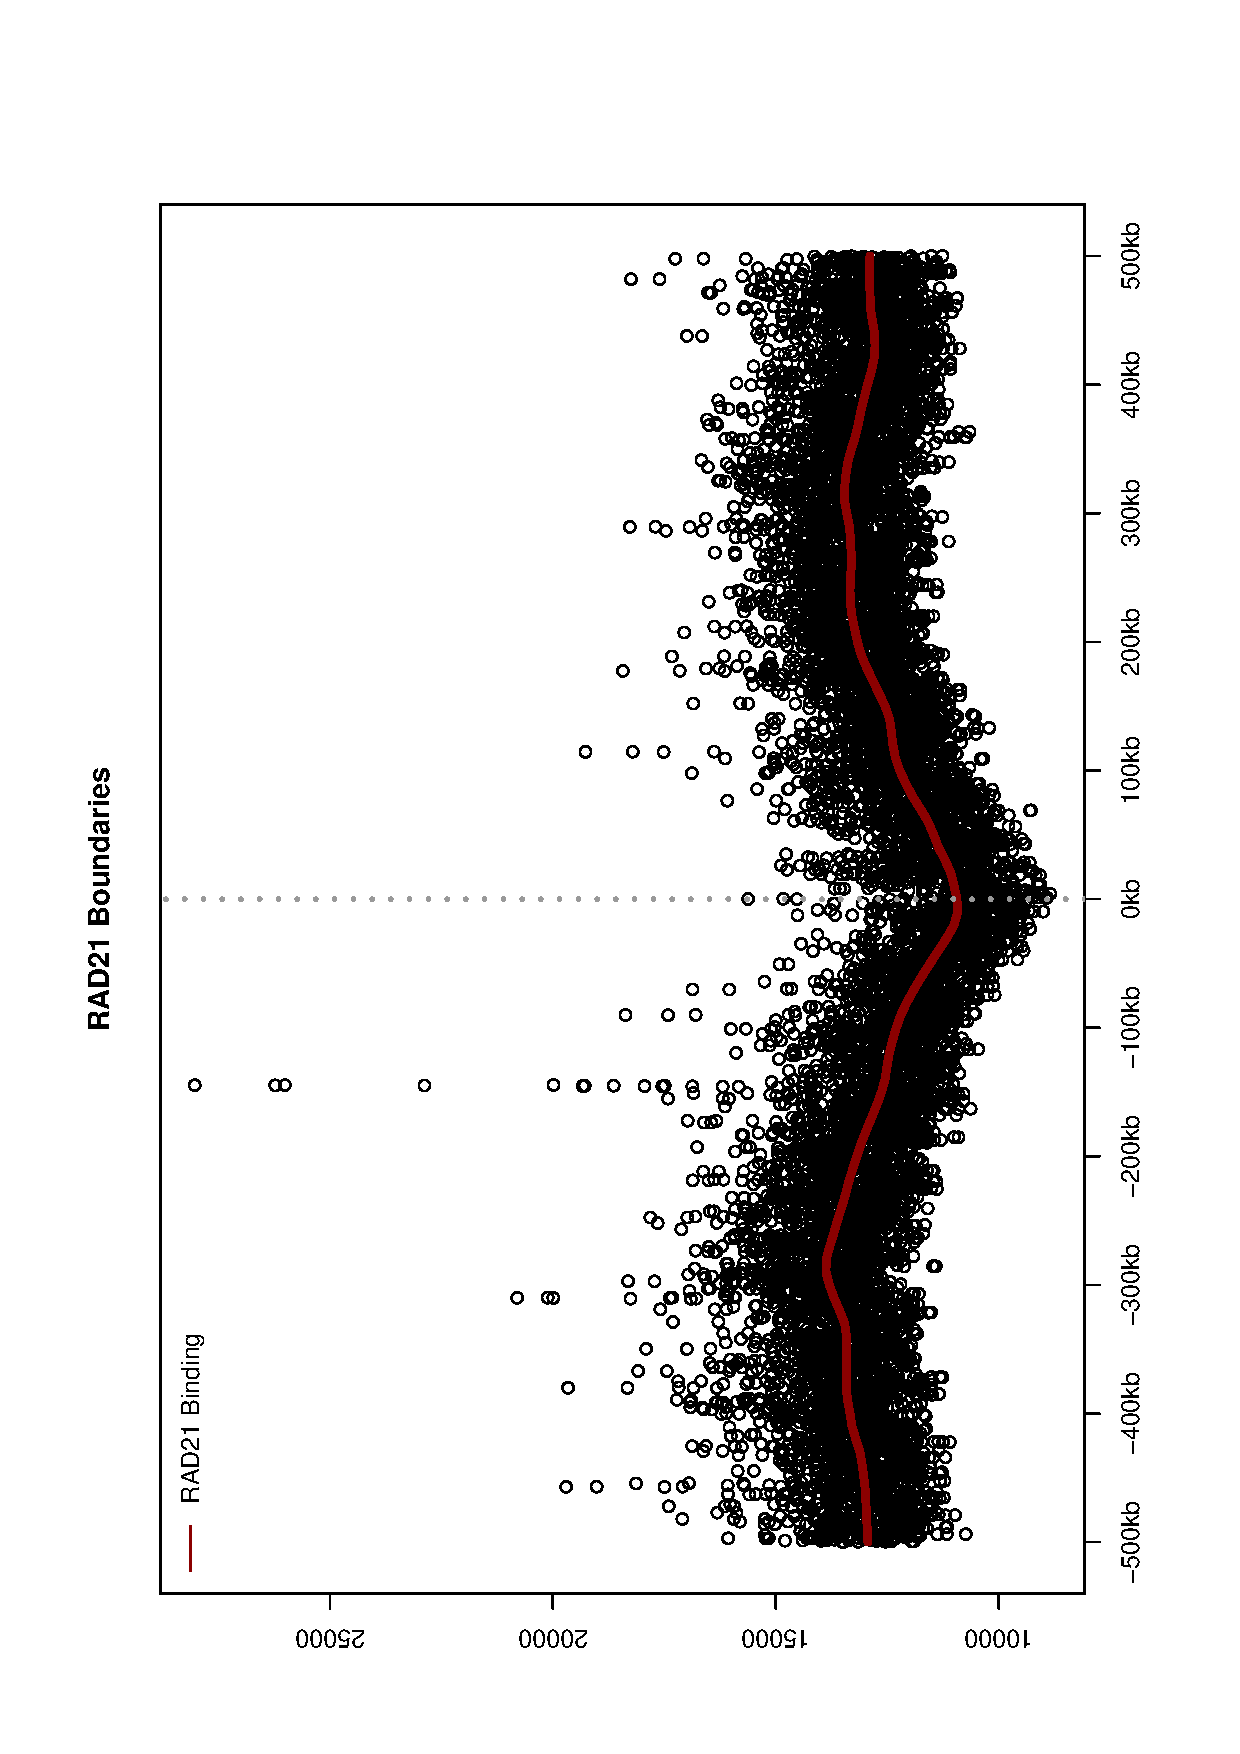
\includegraphics[width=\textwidth]{./figures/supplementary/biomarkers/rad21400kbboundaries.pdf}
  \end{minipage}
  \medskip
  \small
  Binding of various biomarkers around domain boundaries.  Using domains discovered at 200kb (left) and 400kb (right)
  \gls{DI} window sizes, we see peaks in RAD21 and MAFK proteins.  These lend credibility to the theory that 
  these domains play a physiologically relevant regulatory role.
\end{figure}
